%
% 2_ggT.tex -- Abschnitt 2 ggT berechnung mit der Tableau Methode
%
% (c) 2026 Jakob Gierer, OST Ostschweizer Fachhochschule
%
% !TEX root = ../../buch.tex
% !TEX encoding = UTF-8
%
\section{Grösster gemeinsamer Teiler (ggT)
\label{resultante:section:ggT}}
\kopfrechts{Grösster gemeinsamer Teiler}
\subsubsection{ggT in der Tableau-Methode
\label{resultante:subsubsection:tableau}}
Die Tableau-Methode entsteht aus dem euklidischen Algorithmus, für den
\index{euklidischer Algorithmus}%
man die Polynomdivision als Tableau schreibt.
\index{Polynomdivision}%
Die Berechnung des grössten gemeinsamen Teilers von \(a(X)\) und \(b(X)\)
mit \(n = \deg (a) \geq m = \deg (b)\) in der Tableau-Methode beginnt
mit der Sylvester-Matrix \(\syl(b,a)\).
Das ist die Matrix aus Definition \ref{resultante:definition:Sylvester},
in der alle \(m\) Zeilen des \(a(X)\)-Polynoms mit denen des
\(b(X)\)-Polynoms vertauscht werden.
Auf diese Matrix werden nun \(n-m+1\)-Gauss-Zeilenoperationen angewandt.
Die Zeilenoperationen führen im Wesentlichen zu einer Polynomdivision,
\index{Zeilenoperation}%
wie das der euklidische Algorithmus ebenfalls macht.
In den unteren \(m\) Zeilen, an der Stelle der \(a(X)\)-Polynome, entsteht
der entsprechende Rest \(r(X)\) (grüne Zeilen) der Division von \(a(X)\)
und \(b(X)\).
Um nun auf die Stufenform der Sylvester-Matrix zurück zu kommen,
\index{Stufenform}%
werden auf den Restpolynomen zusätzliche Zeilenoperationen angewandt,
bis der Rest sich auf jeder Zeile wiederholt.
Des Weiteren enthalten die ersten \(n-m+1\) Spalten Nullen:
\begin{equation*}
    \centering
    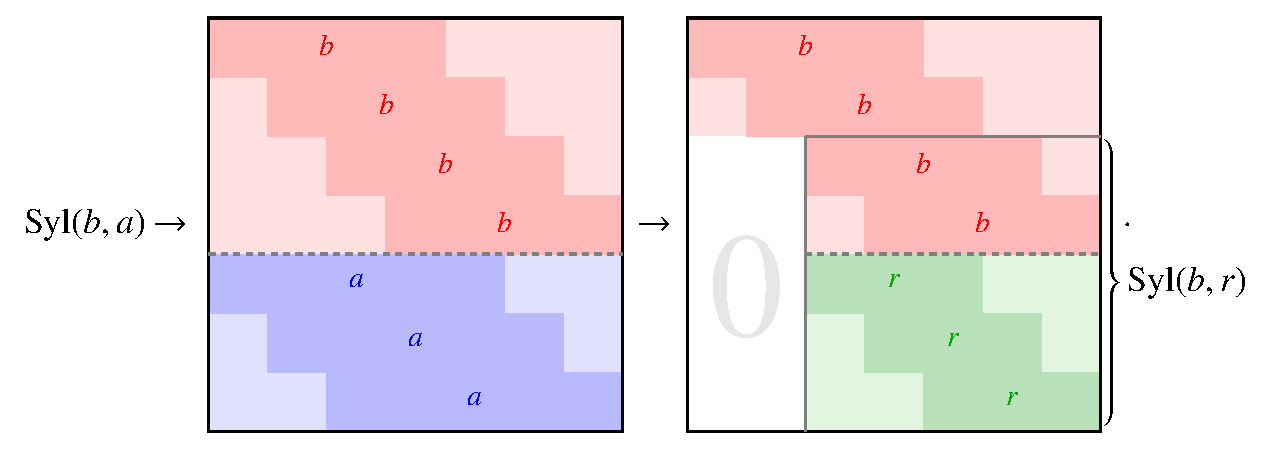
\includegraphics[width=\textwidth]{papers/resultante/pictures/SylvesterTableau.pdf}
    \label{resultante:equation:sylvesterTab}
\end{equation*}
In der rechten unteren Ecke ist nun eine kleinere Sylvester-Matrix
\(\syl(b,r)\) entstanden.
Die Polynome in der neuen Sylvester-Matrix werden ebenfalls vertauscht,
dann kann der nächste Rest mit derselben Methode berechnet werden.
Das zeigt das folgende Beispiel.

\begin{beispiel}
    Die Vorgehensweise zur Ermittlung des grössten gemeinsamen
    Teilers wird am Beispiel \(a(X)=4X^4-7X^3+22X^2-24X+5\) und
    \(b(X)=8X^3+8X^2-16X\) gezeigt.
    Im ersten Tableau sind die ersten vier Zeilen Kopien von \(b(X)\)
    und die drei darunter liegenden sind Kopien von \(a(X)\):
    \begin{equation*}
	\def\r#1{\bgroup\color{darkred}#1\egroup}
	\def\b#1{\bgroup\color{blue}#1\egroup}
	\def\g#1{\bgroup\color{darkgreen}#1\egroup}
	\def\l#1{\bgroup\color{gray!20}#1\egroup}
	\def\p{\phantom{-}}
        \begin{NiceArray}{*{7}{r}}[cell-space-limits=3pt]
        \r{8} & \r{8}  & \r{-16} & \r{0}   & \l{0}   & \l{0}   & \p\l{0} \\
        \l{0} & \r{8}  & \r{8}   & \r{-16} & \r{0}   & \l{0}   & \l{0} \\
        \l{0} & \l{0}  & \r{8}   & \r{8}   & \r{-16} & \r{0}   & \l{0} \\
        \l{0} & \l{0}  & \l{0}   & \r{8}   & \r{8}   & \r{-16} & \r{0} \\
        \b{4} & \b{-7} & \b{22}  & \b{-24} & \b{5}   & \l{0}   & \l{0} \\
        \l{0} & \b{4}  & \b{-7}  & \b{22}  & \b{-24} & \b{5}   & \l{0} \\
        \l{0} & \l{0}  & \b{4}   & \b{-7}  & \b{22}  & \b{-24} & \b{5} 
        \CodeAfter
            \tikz {
                \draw ([xshift=-4pt,yshift=1pt]1-|1)
			rectangle ([xshift=4pt,yshift=-1pt]8-|8);
                \draw[dashed] ([xshift=-4pt,yshift=1pt]5-|1)
			-- ([xshift=4pt,yshift=1pt]5-|8);
            }
        \end{NiceArray}
        \quad\to\quad
        \begin{NiceArray}{*{7}{r}}[cell-space-limits=3pt]
        \r{1} & \p\r{1} & \r{-2} & \r{0}   & \l{0}  & \l{0}  & \p\l{0} \\
        \l{0} & \r{1}   & \r{1}  & \r{-2}  & \r{0}  & \l{0}  & \l{0}   \\
        \l{0} & \l{0}   & \r{1}  & \r{1}   & \r{-2} & \r{0}  & \l{0}   \\
        \l{0} & \l{0}   & \l{0}  & \r{1}   & \r{1}  & \r{-2} & \r{0}   \\
        \l{0} & \l{0}   & \g{41} & \g{-46} & \g{5}  & \l{0}  & \l{0}   \\
        \l{0} & \l{0}   & -11    & 30      & -24    & 5      & \l{0}   \\
        \l{0} & \l{0}   & 4      & -7      & 22     & -24    & 5
        \CodeAfter
            \tikz {
                \draw ([xshift=-4pt,yshift=1pt]1-|1)
			rectangle ([xshift=4pt,yshift=-1pt]8-|8);
                \draw[dashed] ([xshift=-4pt,yshift=1pt]5-|1)
			-- ([xshift=4pt,yshift=1pt]5-|8);
            }
        \end{NiceArray}
	\;\;.
        %\label{resultante:equation:step1}
    \end{equation*}
    Die Stufenform wird wieder hergestellt, indem noch weitere
    Zeilenoperationen auf den letzten zwei Zeilen angewandt werden:
    \begin{equation*}
	\def\r#1{\bgroup\color{darkred}#1\egroup}
	\def\b#1{\bgroup\color{blue}#1\egroup}
	\def\g#1{\bgroup\color{darkgreen}#1\egroup}
	\def\l#1{\bgroup\color{gray!20}#1\egroup}
	\def\p{\phantom{-}}
        \begin{NiceArray}{*{7}{r}}[cell-space-limits=3pt]
        \r{1} & \p\r{1} & \r{-2} & \r{0}   & \l{0}   & \l{0}   & \p\l{0} \\
        \l{0} & \r{1}   & \r{1}  & \r{-2}  & \r{0}   & \l{0}   & \l{0} \\
        \l{0} & \l{0}   & \r{1}  & \r{1}   & \r{-2}  & \r{0}   & \l{0} \\
        \l{0} & \l{0}   & \l{0}  & \r{1}   & \r{1}   & \r{-2}  & \r{0} \\
        \l{0} & \l{0}   & \g{41} & \g{-46} & \g{5}   & \l{0}   & \l{0} \\
        \l{0} & \l{0}   & \l{0}  & \g{41}  & \g{-46} & \g{5}   & \l{0} \\
        \l{0} & \l{0}   & \l{0}  & \l{0}   & \g{41}  & \g{-46} & \g{5}
        \CodeAfter
            \tikz {
                \draw ([xshift=-4pt,yshift=1pt]1-|1)
			rectangle ([xshift=4pt,yshift=-1pt]8-|8);
                \draw[dashed] ([xshift=3pt,yshift=1pt]3-|3)
			-- ([xshift=3pt,yshift=-1pt]8-|3);
                \draw[dashed] ([xshift=3pt,yshift=1pt]3-|3)
			-- ([xshift=4pt,yshift=1pt]3-|8);
                \draw[dashed] ([xshift=3pt,yshift=1pt]5-|3)
			-- ([xshift=4pt,yshift=1pt]5-|8);
            }
        \end{NiceArray}
	\;\;.
        %\label{resultante:equation:step2}
    \end{equation*}
    Im kleineren Tableau unten rechts steht das Polynom \(b(X)\) oben
    und darunter das Rest-polynom \(r(X)=r_1(X)=41X^2-46X+5\).
    Nun werden die beiden Bereiche vertauscht und dieselbe Methode wiederholt:
    \begin{equation*}
	\def\l#1{\bgroup\color{gray!20}#1\egroup}
	\def\p{\phantom{-}}
        \begin{NiceArray}{*{5}{r}}[cell-space-limits=3pt]
        41    & -46   & 5   & \l{0} & \p\l{0} \\
        \l{0} & 41    & -46 & 5     & \l{0}   \\
        \l{0} & \l{0} & 41  & -46   & 5       \\
        1     & 1     & -2  & 0     & \l{0}   \\
        \l{0} & 1     & 1   & -2    & 0
        \CodeAfter
            \tikz {
                \draw ([xshift=-3pt,yshift=1pt]1-|1) rectangle ([xshift=4pt,yshift=-1pt]6-|6);
                \draw[dashed] ([xshift=-3pt,yshift=1pt]4-|1) -- ([xshift=4pt,yshift=1pt]4-|6);
            }
        \end{NiceArray}
        \quad\to\quad
        \begin{NiceArray}{*{5}{c}}[cell-space-limits=3pt]
        1     & -\frac{46}{41} & \p\frac{5}{41}     & \l{\p0}            & \l{\p0} \\
        \l{0} & 1              & -\frac{46}{41}     & \p\frac{5}{41}     & \l{\p0} \\
        \l{0} & \l{0}          & \p1                & -\frac{46}{41}     & \p\frac{5}{41} \\
        \l{0} & \l{0}          & \p\frac{435}{1681} & -\frac{435}{1681}  & \l{\p0} \\
        \l{0} & \l{0}          & \l{\p0}            & \p\frac{435}{1681} & -\frac{435}{1681}
        \CodeAfter
            \tikz {
                \draw ([xshift=-4pt,yshift=1pt]1-|1) rectangle ([xshift=3pt,yshift=-1pt]6-|6);
                \draw[dashed] ([xshift=1pt]3-|3) -- ([xshift=1pt,yshift=-1pt]6-|3);
                \draw[dashed] ([xshift=1pt]3-|3) -- ([xshift=3pt]3-|6);
                \draw[dashed] ([xshift=1pt]4-|3) -- ([xshift=3pt]4-|6);
            }
        \end{NiceArray}
	\;\;.
        %\label{resultante:equation:step3}
    \end{equation*}
    Erneut ist der Rest \(r_2(X)=\frac{435}{1681}X-\frac{435}{1681}\) in den unteren Zeilen zu finden.
    Der Subbereich wird wieder vertauscht und der Rest bestimmt:
    \begin{equation*}
	\def\r#1{\bgroup\color{darkred}#1\egroup}
	\def\b#1{\bgroup\color{brown}#1\egroup}
	\def\g#1{\bgroup\color{darkgreen}#1\egroup}
	\def\l#1{\bgroup\color{gray!20}#1\egroup}
	\def\p{\phantom{-}}
        \begin{NiceArray}{*{3}{c}}[cell-space-limits=3pt]
        \g{\frac{435}{1681}} & \g{-\frac{435}{1681}} & \l{\phantom{-}0} \\
        \l{0} & \g{\p\frac{435}{1681}} & \g{-\frac{435}{1681}} \\
        \b{1} & \b{-\frac{46}{41}}     & \b{\p\frac{5}{41}}
        \CodeAfter
            \tikz {
                \draw ([xshift=-3pt,yshift=1pt]1-|1)
			rectangle ([xshift=3pt,yshift=-1pt]4-|4);
                \draw[dashed] ([xshift=-3pt]3-|1) -- ([xshift=3pt]3-|4);
            }
        \end{NiceArray}
        \quad\to\quad
        \begin{NiceArray}{*{3}{r}}[cell-space-limits=3pt]
        \g{1} & \g{-1} & \l{0}  \\
        \l{0} & \g{1}  & \g{-1} \\
        \l{0} & \l{0}  & \b{0}
        \CodeAfter
            \tikz {
                \draw ([xshift=-4pt,yshift=1pt]1-|1)
			rectangle ([xshift=4pt,yshift=-1pt]4-|4);
                \draw[dashed] ([xshift=1.5pt,yshift=1pt]3-|3)
			-- ([xshift=1.5pt,yshift=-1pt]4-|3);
                \draw[dashed] ([xshift=-4pt,yshift=1pt]3-|1)
		-- ([xshift=4pt,yshift=1pt]3-|4);
            }
        \end{NiceArray}
	\;\;.
        %\label{resultante:equation:step4}
    \end{equation*}
    Aus dem Schlusstableau kann der verbleibende Rest \(r_3(X)=0\)
    herausgelesen werden.
    In der Zeile darüber ist der normierte grösste gemeinsame Teiler,
    was dem Rest aus dem vorherigen Schritt entpricht.
    Somit ist \(X-1\) der grösste gemeinsame Teiler von \(a(X)\) und \(b(X)\).
    \label{resultante:beispiel:ggt}
\end{beispiel}

Diese Methode ermöglicht, den grössten gemeinsamen Teiler zu bestimmen.
Da sich die Polynome \(a(X)\) und \(b(X)\) bzw. \(b(X)\) und \(r(X)\)
in der Sylvester-Matrix jeweils um eine Spalte verschoben wiederholen
müssen, reicht es aus, die erste Zeile auf das Pivotelement zu normieren
und auf die restlichen Zeilen des Polynoms zu kopieren.
Ausserdem können weitere Zeilenoperationen eingespart werden, indem
nur die erste Zeile des Restes berechnet und auf die darunter liegenden
Zeilen verschoben kopiert wird.


\subsubsection{Die Determinante der Sylvester-Matrix
\label{resultante:subsubsection:determ}}

Die Vertauschung von Zeilen und die Zeilenoperationen selbst, die zur
Berechnung des Restes der Sylvester-Matrix nötig sind, ändern die
Determinante der Sylvester-Matrix nicht.
Lediglich werden \(nm\) Vertauschungen für die Methode benötigt, daher folgt
\begin{equation}
    \det(\syl(a,b))=(-1)^{nm}\det(\syl(b,a)).
    \label{resultante:equation:detsyl}
\end{equation} 
Es kann also höchstens zu einem Wechsel des Vorzeichens der Determinante kommen.

Der Algorithmus zur Berechnung der Determinante endet, sobald der grüne
Rest \(=0\) ist oder im braunen Feld (\(?\)-Feld) eine Zahl stehen bleibt.
Ist der Rest \(=0\), ist in der darüber liegenden Zeile der grösste
gemeinsame Teiler ein Polynom vom Grad \(\geq1\):
\begin{equation*}
    \centering
    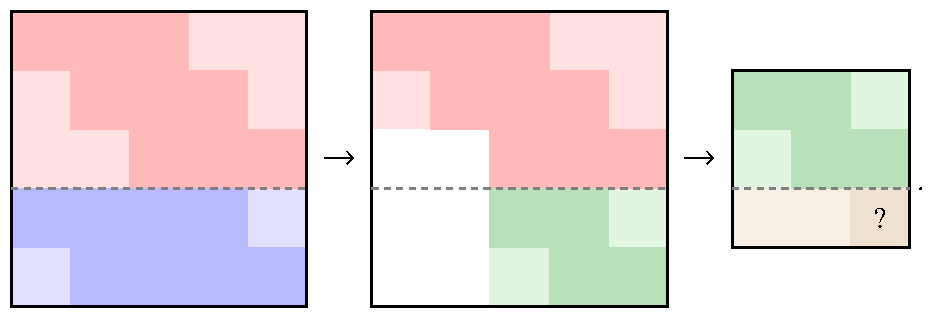
\includegraphics[width=0.8\textwidth]{papers/resultante/pictures/FinalTableau.pdf}
    \label{resultante:equation:finalTab}
\end{equation*}
Falls der letzte Rest im braunen Feld \(\neq0\) übrig bleibt, ist
der grösste gemeinsame Teiler \(=1\), die beiden Polynome \(a(X)\)
und \(b(X)\) sind somit teilerfremd.

Daraus lässt sich ablesen, dass die Determinante genau dann von Null
verschieden ist, wenn die beiden Polynome teilerfremd sind.
\begin{satz}[Resultante und Teiler]
    Zwei Polynome \(f(X)\) und \(g(X)\) sind genau dann teilerfremd,
    wenn \(\det(\syl(f,g))\neq0\) ist.
\end{satz}
\begin{definition}[Resultante]
    Wie bereits in der Einleitung
    (Abschnitt~\ref{resultante:equation:definition})
    geschrieben: Sind \(f\) und \(g\) Polynome, dann heisst die Determinante
    der Sylvester-Matrix
    \begin{equation*}
        \Res(f,g)=\det(\syl(f,g))
    \end{equation*}
    die \emph{Resultante} der Polynome.
    \label{resultante:definition:resultante}
\end{definition}

Folglich ist die Resultante zweier Polynome genau dann gleich Null,
wenn sie eine gemeinsame Nullstelle haben.

Das Beispiel \ref{resultante:beispiel:ggt} zeigt: Die Berechnung der
Resultante lässt sich bereits mit grund\-legenden Werkzeugen der linearen
Algebra umsetzen.
